\subsection{Opcje startowe}\label{sub:uruchamianie programu}
\paragraph{}
Opcje wiersza poleceń możemy łatwo wylistować uruchamiając program z parametrem -h lub --help. Oto one:

\begin{description}
\item[-r (--resolution) xres yres] Ustawia rozdzielczość programu na podaną w parametrze.
\item[-f (--fullscreen) {true|false}] włącza lub wyłącza (opcja domyślna) tryb pełnoekranowy.
\item[--deffered.textures {true|false}] włącza (opcja domyślna) lub wyłącza teksturowanie planet.
\item[--deffered.lighting {true|false}] włącza (opcja domyślna) lub wyłącza oświetlenie.
\item[--deffered.lights\_range arg] ustawia zasięg świateł.
\item[--deffered.normals {true|false}] opcja debugowa, wyświetla normalne zamiast kolorów - domyślnie wyłączone.
\item[--deffered.brightness arg] ustawia jasność światła otoczenia.
\item[--trace.enable {true|false}] włącza lub wyłącza (opcja domyślna) ślad pozostawiany przez planety.
\item[--trace.frequency arg] ustawia częstotliwość stawiania śladu (w sekundach).
\item[--trace.length arg] ustawia ilość śladów które zostawia planeta
\end{description}

\subsection{Poruszanie kamerą}\label{sub:poruszanie kamerą}
\paragraph{}
Kamera w aplikacji jest swobodna, co oznacza, że możemy poruszać i obracać nią we wszystkich kierunkach. Do przesuwania kamery w przód i w tył służą odpowiednio klawisze W i S. Przesunięcia w lewo i w prawo odbywają się przy pomocy klawiszy A i D, natomiast ruch w górę i w dół jest możliwy przy użyciu klawiszy Q i E. Tę ostatnią czynność możemy zrealizować także korzystając z klawisza Ctrl i spacji.
\paragraph{}
Do wykonywania obrotów należy użyć myszy. Jest ona używana także do korzystania z GUI. Do odróżnienia tych dwu czynności używany jest prawy przycisk myszy. Kiedy jest on wciśnięty, ruchy myszką odpowiadają "rozglądaniu się" w przestrzeni kosmicznej. 
\paragraph{}
Dodatkowo, jeżeli chcemy śledzić jakąś planetę, a nie chce nam się ciągle lecieć za nią kamerą, wystarczy, że klikniemy na nią lewym klawiszem myszy. Wówczas kamera automatycznie będzie zmieniała swoje położenie tak, aby nie zmieniać odległości od zaznaczonej planety. Aby wrócić do swobodnego trybu kamery, wystarczy kliknąć gdzieś w przestrzeń kosmiczną.

\subsection{Interfejs graficzny}\label{sub:interfejs graficzny}
\paragraph{}

Po uruchomieniu aplikacji pokazuje się okno przedstawiające kosmos. Na nim znajdują się również guziki. Przy ich pomocy możliwe jest wczytanie bądź zapisanie układu planet. Można również wystartować lub zatrzymać animację. Dostępne są też różne opcje programu, takie jak modyfikacji szybkości kamery, szybkości animacji oraz inne opcje graficzne i fizyczne. W tym rozdziale przedstawione będzie użycie podstawowych możliwości GUI. Dla oszczędności tuszu, kolory na obrazkach są odwrócone w porównaniu do oryginalnej aplikacji.

\begin{figure}[ht!]
\centering
\fbox{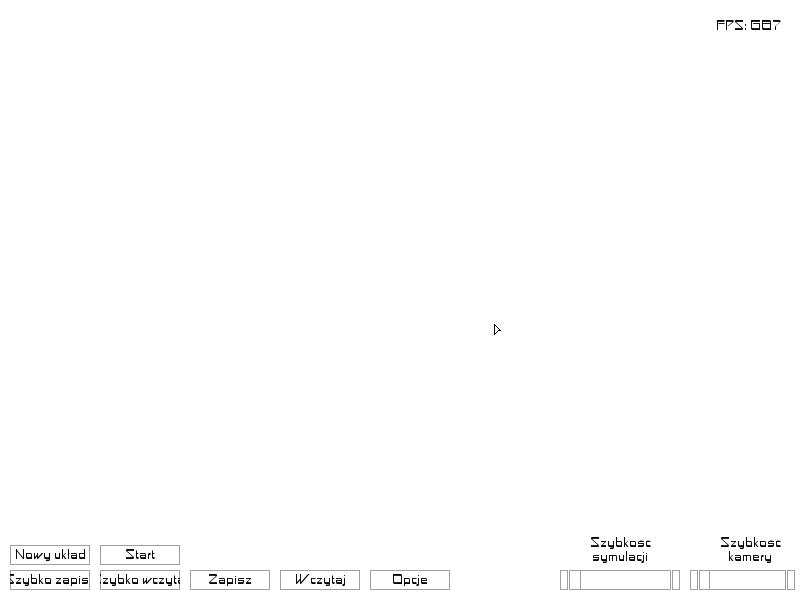
\includegraphics[width=0.75\textwidth]{img/inst_00.png}}
\caption{Początkowe okno}
\label{fig:inst_00}
\end{figure}

\subsubsection{Odczyt}\label{ssub:odczyt}
\paragraph{}

Po wciśnięciu guzika wczytaj, na ekranie pojawi się okno wczytywania. Możemy na nim wybrać interesujący nas układ. Po wybraniu układu oraz wciśnięciu "Wczytaj" układ zostanie załadowany. Można również wcisnąć guzik "Szybko wczytaj" który pozwoli na natychmiastowe wczytanie układu o nazwie "qsave.sav".

\begin{figure}[ht!]
\centering
\fbox{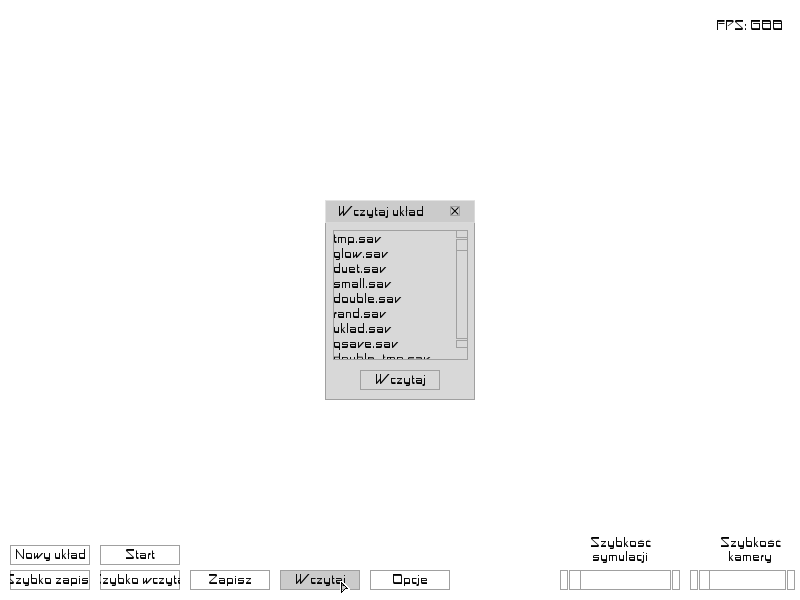
\includegraphics[width=0.75\textwidth]{img/inst_06.png}}
\caption{Okno wczytywania}
\label{fig:inst_01}
\end{figure}

\begin{figure}[ht!]
\centering
\fbox{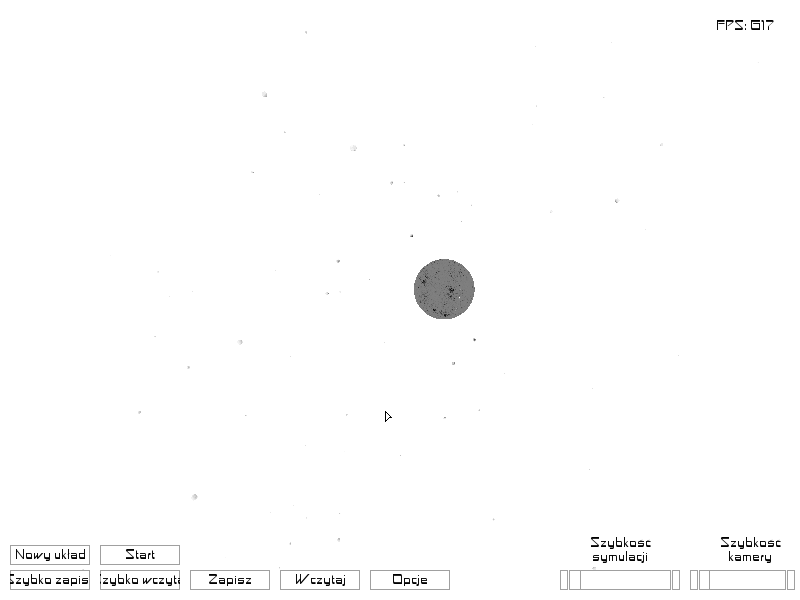
\includegraphics[width=0.75\textwidth]{img/inst_02.png}}
\caption{Wczytany układ}
\label{fig:inst_02}
\end{figure}

\subsubsection{Start animacji}\label{ssub:start animacji}
\paragraph{}

Układ domyślnie wczytywany jest w trybie pauzy. Aby wystartować animację należy wcisnąć guzik start. Powinien on w tedy zmienić nazwę i funkcję na puaza, a planety powinny zacząć się poruszać.

%\begin{figure}[ht!]
%\centering
%\fbox{\includegraphics[width=0.75\textwidth]{img/inst_03.png}}
%\caption{Animacja}
%\label{fig:inst_03}
%\end{figure}

\subsubsection{Zapis układu}\label{ssub:zapis ukladu}
\paragraph{}

Jeżeli aktualny stan układu się nam podoba, możemy go zapisać. Należy w tym celu wcisnąć guzik "Zapisz", po wciśnięciu którego na ekranie pojawi się okno. W oknie tym należy wpisać nazwę nowego układu, oraz wcisnąć guzik "Zapisz" na oknie. Od tej pory nowy układ będzie dostępny do wczytania przez aplikację.


\begin{figure}[ht!]
\centering
\fbox{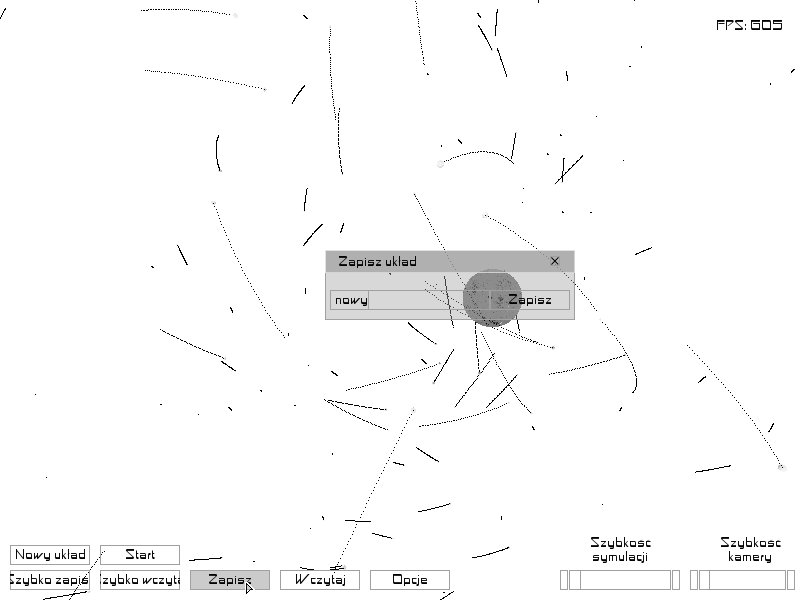
\includegraphics[width=0.75\textwidth]{img/inst_07.png}}
\caption{Okno zapisu}
\label{fig:inst_04}
\end{figure}

\subsubsection{Opcje}\label{ssub:opcje}
\paragraph{}

Na głównym ekranie znajdują się również dwa suwaki, którymi można zmieniać odpowiednio prędkość symulacji, oraz szybkość kamery. Pierwszy suwak odpowiada za liczbę klatek fizyki na jedną klatkę programu. Drugi natomiast zmienia szybkość poruszania kamery w przestrzeni. Dodatkowo po wciśnięciu guzika "Opcje" który znajduje się w głównym ekranie aplikacji, jest dostęp do dodatkowych opcji programu. Można tam manipulować ustawieniami graficznymi, fizycznymi i innymi.

